%!TEX program  = xelatex
\documentclass{cumcmthesis}
\usepackage{float}
\begin{document}

\section{Mediachain元数据区块链模型}

\subsection{Mediachain模型综述}
Mediachain是美国Mediachain Labs公司开发的一种基于区块链技术的开源数字媒体版权保护机制。它的核心产品是一个元数据协议,通过它内容创作者可以给自己的作品附加信息,并把该数据打上时间戳放到对应的的区块链里,然后放到InterPlanetary File System(IPFS,吸收了区块链技术的分布式文件系统)上。其特点主要有如下几点:

(1)安全。Mediachain系统中的每个对象都是可寻址的和自我认证的,这意味着数据可以被多个不可信的参与者复制和使用,同时还能保持不可篡改性,因为数据完整性是通过加密认证的。

(2)可扩展。Mediachain规定了一个可扩展的元数据纲要(schema),使得数字媒体的元数据存储变得规范化并且调和不同的元数据,从而使对象之间的丰富关系可以用merkle DAGs表示。
这使得应用程序层可以根据用户的需求进行表达,且在系统中可以通过多种非破坏性的方式使用内容地址链接来引用或扩展数据。

(3)低成本。Mediachain采用点对点的去中心化的分布式数据库存储信息。所有数据都是定位的,任何人都能以安全的方式复制和服务他人的数据集,这降低了参与者的成本,并增加了访问数据时的带宽。

\begin{figure}[!h]
	\centering
	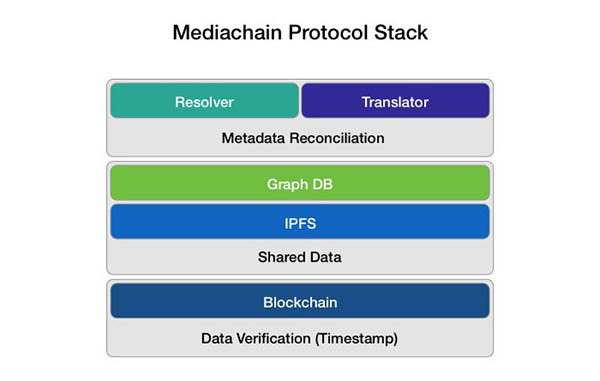
\includegraphics[width=.8\textwidth]{mediachain.jpg}
	\caption{Mediachain协议示意图}
\end{figure}

基于Mediachain的产权追溯流程如下:

step1: 数字版权所有者(一般是作者)加入区块链时,Mediachain会分配给版权所有者独一无二的Publisher ID(发布者ID),通过Publisher ID同时IPFS系统会通过非对称加密算法为版权所有者生成公钥和私匙,对公匙使用哈希方法生成peer地址。

step2: 当版权所有者想要发布数字媒体作品时,需要首先构建作品的声明信息,声明信息包括了指向作品元数据和纲要数据的索引,发行方的签名,时间戳,作品的分类,之后声明信息会随着加密货币被记录在区块链上,并且由时间戳构成防伪标志。这些声明信息会被记录员记录在区块链主链上,而作品的元数据则被发行方存储到自己的IPFS系统里。

step3: 版权所有者可以通过添加peer地址,之后使用Mediachain提供的合并机制把其他版权方的数字版权元数据合并到自己的IPFS分布式数据库里。网络上的peer地址里的元数据未必可信,这使得虽然有区块链主链保证声明的真实性,但直接访问整个IPFS网络会下载无意义的元数据,所以Mediachain允许使用者可以仅添加可信的peer地址来节约空间。

step4: 数字版权的使用者如果想使用这个数字作品,首先需要拥有数字作品的元数据,之后可搜索已添加的peer地址作为元数据库来源,使得使用者可通过作品元数据反向定位到声明以找到作者,并且在下文的产权交易模型中付费。至此,基于Mediachain数字媒体元数据区块链的产权追溯完成。

\subsection{Publisher ID的生成与Hash算法}
当Mediachain区块链主链上产生"发布声明"时,区块链上各记录员协调后生成的记录的有效性依赖于声明中的数字签名信息和用户对应的Publisher ID的准确性。模型中Publisher ID的构建依赖于hash算法。

\subsubsection{哈希表}

哈希表是根据关键码值(key)进行直接访问的数据结构。即将关键码值映射到表中一个位置来访问相应记录。如给出表M,确定函数f(key),对任意给定的关键字值key,代入函数后得到包含该关键字的记录在表中的地址(address),函数f(key)为即为表M的hash 函数。常见的哈希函数方法包括直接寻址法,数字分析法,随机数法等。

\begin{figure}[!h]
	\centering
	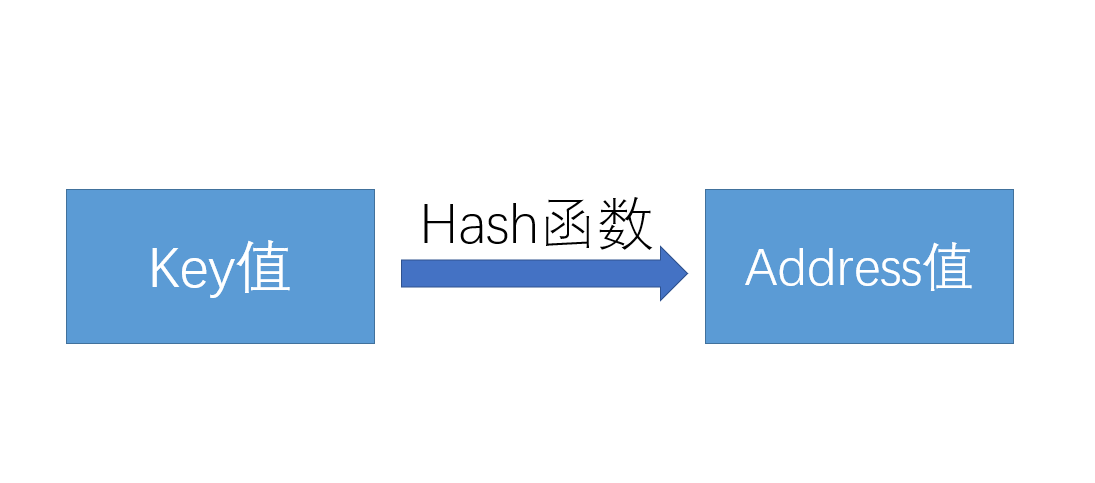
\includegraphics[width=.6\textwidth]{hash.png}
	\caption{hash映射}
\end{figure}

对不同的关键码值可能得到同一散列地址,即 $k1\neq k2$ ,而f(k1)=f(k2),这种现象称为碰撞(Collision)。具有相同函数值的关键字对该散列函数来说称为同义码值。这样的码值破坏了体系的一致性。这时,hash算法应该建立相应的防碰撞机制,例如开放寻址法和再散列法,建立另一个散列函数地址或建立探测散列的机制。同时,也可以加大哈希表的容量,从而增加伪造难度。

哈希表的优势首先在于不可逆性,由相应的地址很难得到对应的关键码值,这为安全性提供了有力的保障。同时,关键码值必须保证完全的准确性,暴力破解者很难完全建立正确的映射。

\subsubsection{SHA-256算法}

SHA-256 算法又称安全散列算法。其输入的最大长度不超过2*64 bit,输入按512-bit 分组进行处理,产生的输出是一个256-bit 的地址。该算法处理如下:

Step1 准备:

处理输入key的长度,使key长度满足mod 512 = 448,并将初始64位初始key值的位长度附加在后面。初始化缓存,使用一个256-bit 的8个缓存器来存放算法函数的中间及最终结果。 将处理后的512-bit(16个字)进行分组。

Step2运算:

使用基本的逻辑函数,进行迭代运算。可由分组之后的key值得到W(i)(i=0,1….15)再通过递推公式新的消息块W(i)(i=16,17….63).

SHA-256基于逻辑函数,每个函数均基于32位字运算,同样的这些函数的计算结果也是一个32位字。用缓存器缓存中间结果记作 ABCDEFGH,循环迭代下面公

$T_{i+1}=H_{i}+\sum_0{E_{i}}+Ch(E_{i},F_{i},G_{i})+K_{i}+W_{i}$

$T_{i+2}=\sum_1{A_{i}+Maj(A_{i}+B_{i}+C_{i})}$

$H_{i+1}=G_{i},G_{i+1}=F_{i},F_{i+1}=E_{i},E_{i+1}=D_{i}+T_{i+1}$

$D_{i+1}=C_{i},C_{i+1}=B_{i},B_{i+1}=A_{i},A_{i+1}=T_{i+1}+T_{i+2}$

W(i)的循环公式为

$W_{i}=W_{i-2}+W_{i-16}+\sum_a(W(i-15)+\sum_b(W(i-2)))$

上述逻辑函数定义如下

$CH( x, y, z) = (x\land y) \oplus  ( (x\land z)$

$Maj( x, y, z) = (x \land y) \oplus (x \land z) \oplus (y \land z)$

$\sum_0(x) = ROTR^{2}(x) \oplus ROTR^{13}(x) \oplus ROTR^{22}(x)$

$\sum_1(x) = ROTR^{6}(x) \oplus ROTR^{11}(x) \oplus ROTR^{25}(x)$

$\sum_a(x) = ROTR^{7}(x) \oplus ROTR^{18}(x) \oplus SHR^{3}(x)$

$\sum_b(x) = ROTR^{17}(x) \oplus ROTR^{19}(x) \oplus SHR^{10}(x)$

\begin{figure}[ht]
	\centering
	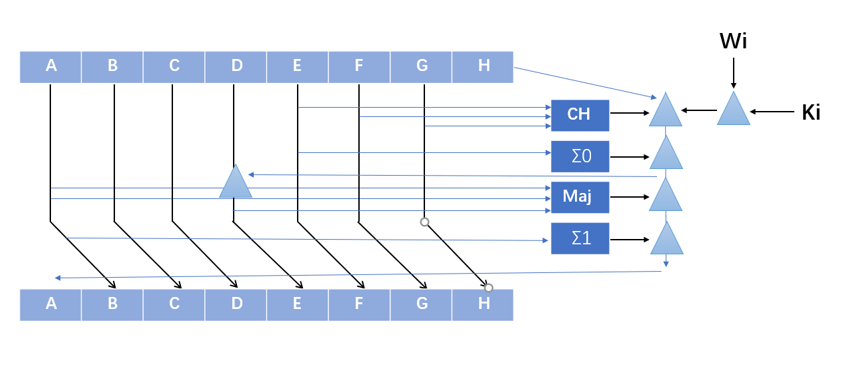
\includegraphics[width=.9\textwidth]{s256.png}
	\caption{SHA256流程图}
\end{figure}
Step3结果:

SHA-256算法最后一次缓存器存放结果产生的输出便是256-bit的address值。\newline

\subsubsection{公钥的生成--对应于Publisher ID}

1.每一个用户都要设置一个密码,由密码通过SHA256算法得到一个256位的数。通过ECC方法作用于这个数得到的码即为用户的公钥。

2.计算公钥的 SHA256 哈希值,并得到其结果的 RIPEMD160 哈希值。运算结束后在前面添加地址号得到前置地址。

注:RIPEMD (RACE Integrity Primitives Evaluation Message Digest,RACE原始完整性校验讯息摘要)是一种加密哈希函数。RIPEMD-160是以原始版RIPEMD所改进的160位元版本,而且是RIPEMD系列中最常见的版本。


3.两次计算 前置地址的 SHA-256 哈希值,取结果的后四个字节作为校验码。将校验码加在前置地址后面,即生成了用户地址的 16 进制结果。

4.将密码对应的sha-256值后面添加版本号(vis)和压缩标志(f)并在末尾添加校验码即生成私钥的 16 进制表示. 

\subsection{ECDH型数字签名}

整个版权交易与资金流通过程中,需要数字签名来建立一个认证机制。

模型中建立了基于椭圆曲线的ECDH数字签名的变体,设消息为m:

step1:签名生成

A.选择椭圆曲线,并确定相应基准点G

B.随机或伪随机的生成一个整数k属于$Z_n^*$,计算kG=(x1,y
1),r1=x1 mod n,r1=0,则

返回重选k

C.e=SHA-256(m)

D.r=r1e mod n,s=k + rd mod n,r=0或s=0,则重选k

step2:签名认证

A.接受者验证(r,s)是A对消息m的签名

B.验证r,s是[1,n-1]中整数

C.计算e=SHA-256(m)

D.X=sG-rQ=(x1,y1),X=0,拒绝这个签名,否则计算v=x1e mod n,只有v=r时认证成功。

\begin{figure}[ht]
	\centering
	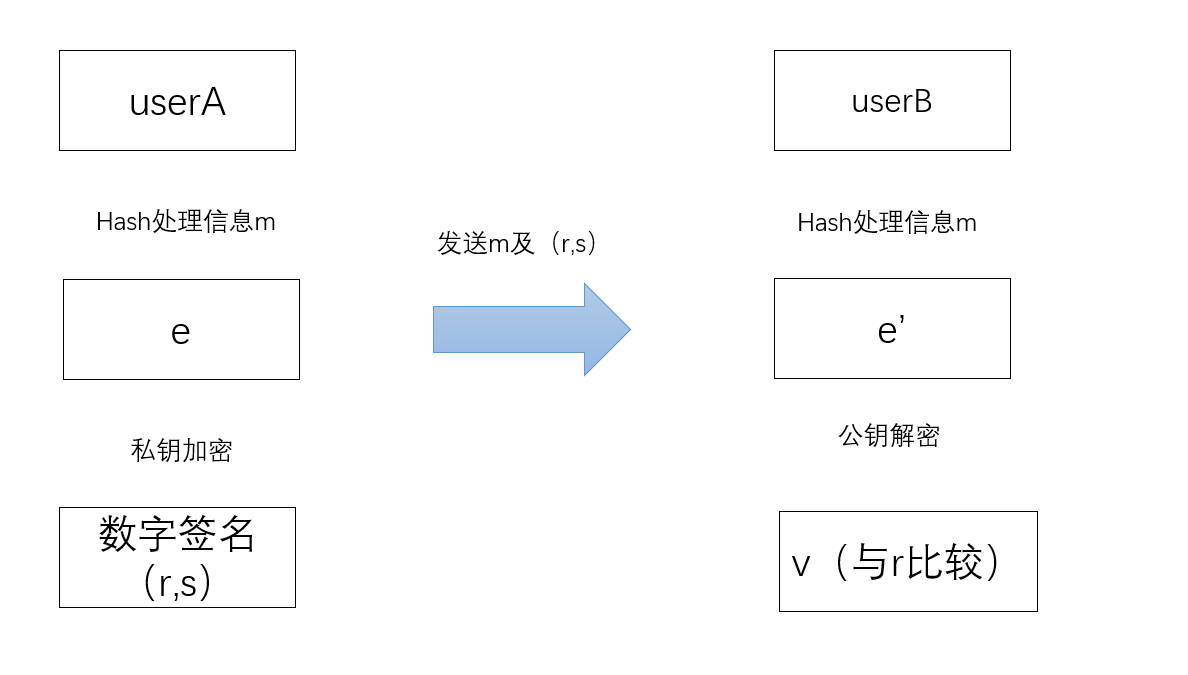
\includegraphics[width=.8\textwidth]{shu.png}
	\caption{数字签名认证}
\end{figure}

\subsection{Mediachain机制详解}
为了将数字作品版权加密存储在比特币区块链中,一般的做法是用OP\_RETURN或CoinSpark制作加密ID保存到区块链中,代表这些集中管理的数据;或者用定制的分布式账本将元数据直接绑定到每笔交易中。但这两种将元数据加密加入区块链的方法都有各自的缺点。比特币协议的OP\_RETURN内置代码每笔交易允许的最大数据容量是40字节,这样在区块链中存储更多元数据串就很难。于是,这种方法的效率就很低。第二个方法的缺陷在于其安全性。缺乏矿工和算力的新建网络对51\%攻击毫无抵抗力。一旦区块链和数据量扩展,保护数据安全的算力就更加紧张。

Mediachain并不依赖区块链的内置功能来存储元数据,采取了一种无需大量存储数据就可以验证数据的新方法,即通过声明来验证数据。

\begin{figure}[!h]
	\centering
	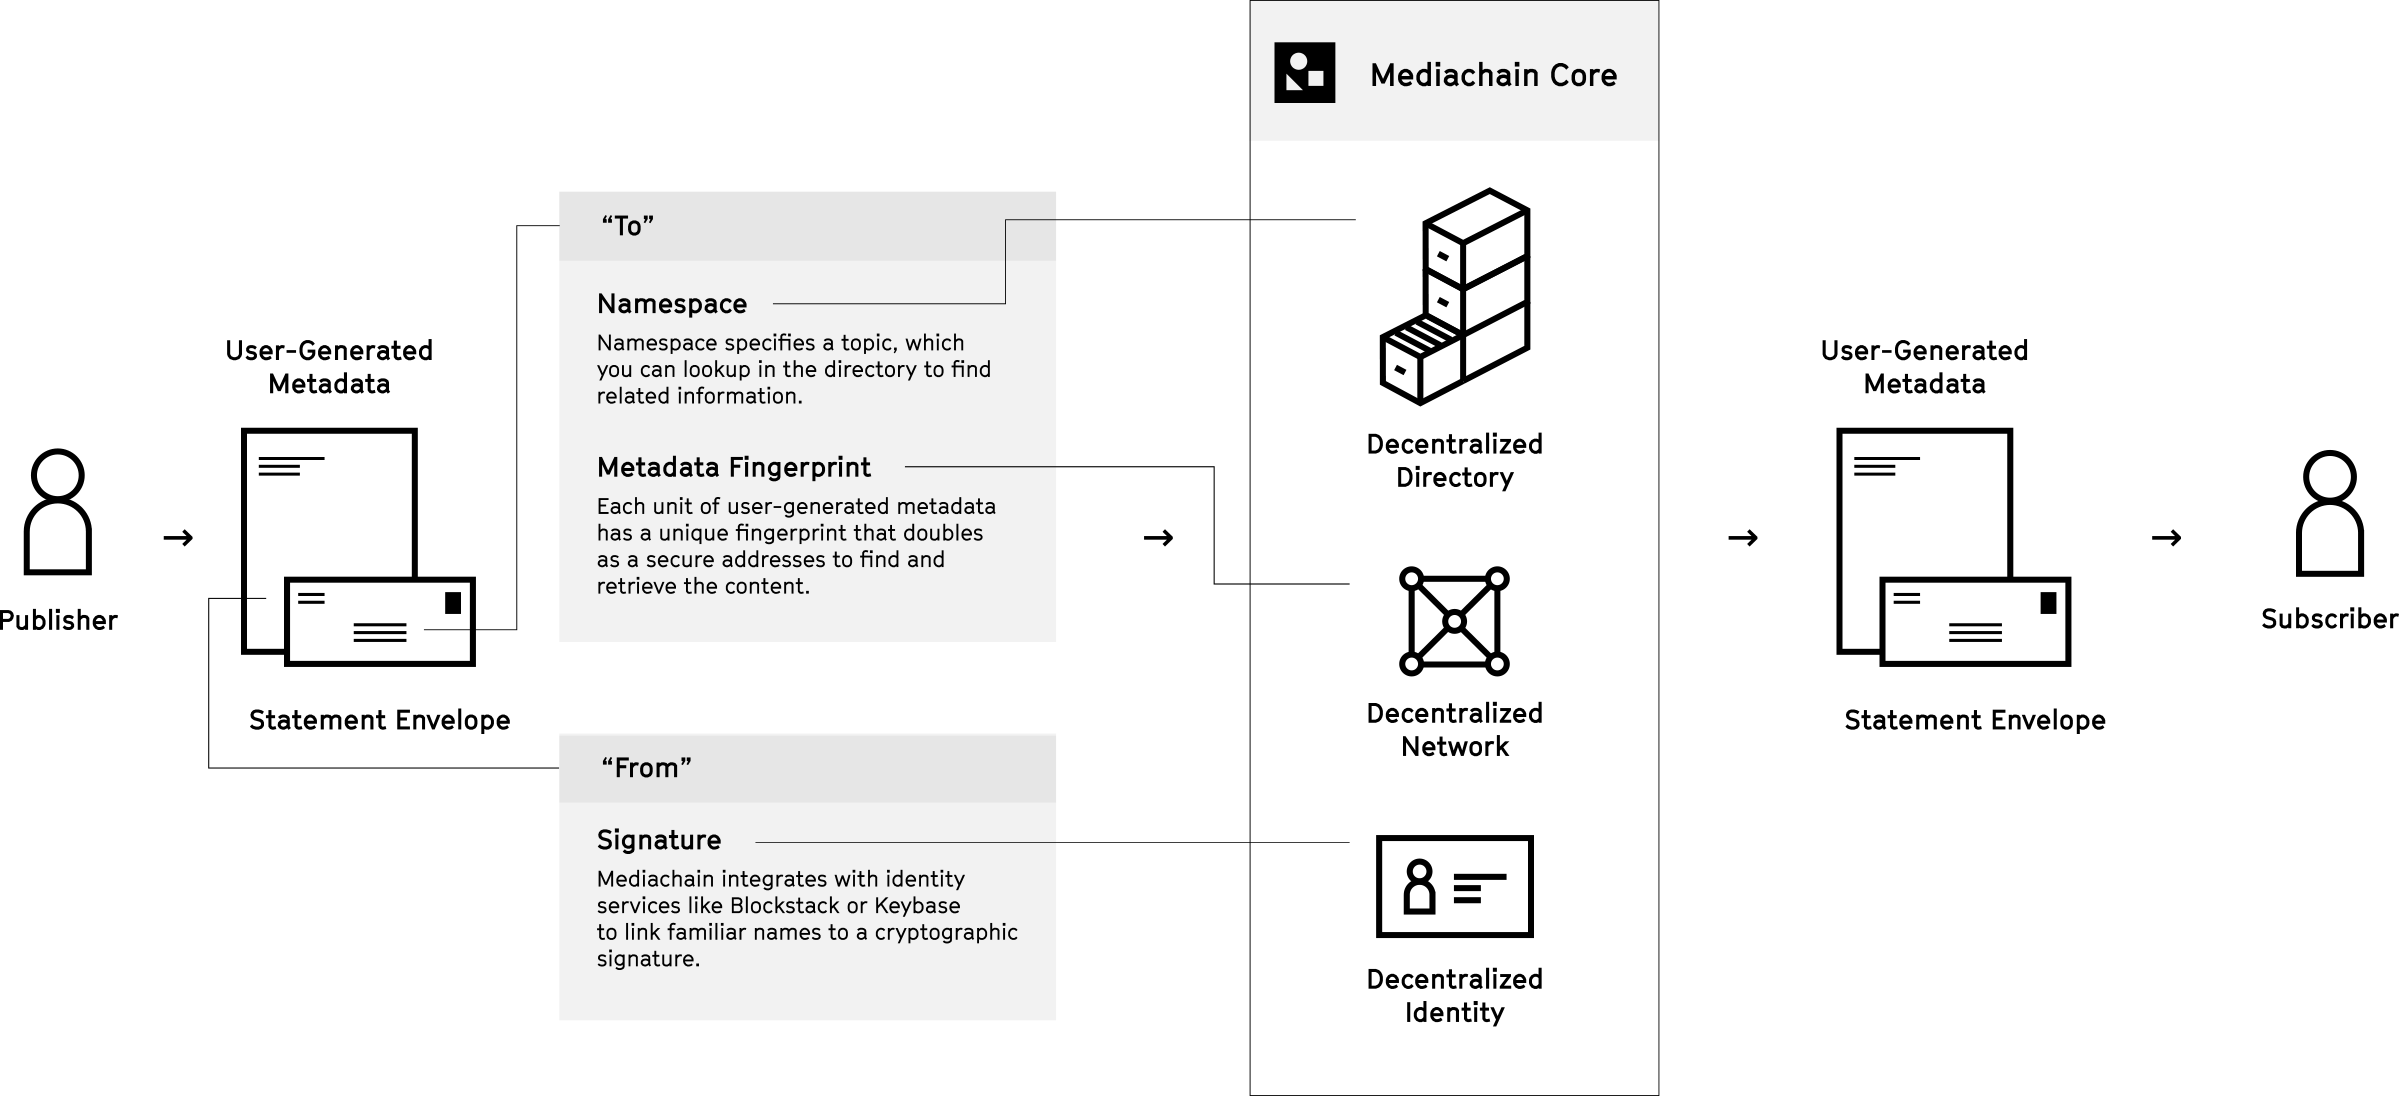
\includegraphics[width=.8\textwidth]{mc-stack.png}
	\caption{声明与元数据的关系类似于信封和信}
\end{figure}

在创建一个声明之前,必须先创建元数据文件,元数据文件包括了数字媒体作品的所有属性,包括创作时间,作者等等。之后还要创建元数据纲要文件,这个文件规定了上面提及的数字媒体属性分别是什么类别的,例如作者姓名是以字符串方式存储大小限制为8B,发表日期是以整数方式存储。作者在创建元数据文件和元数据纲要文件时均会使用SHA2-256算法生成唯一的哈希。命名空间则是一个独立的逻辑空间,使得Mediachain参与者不需要借助任何外部索引即可通过命名空间检索同类的作品版权声明,这使得IPFS系统中不同的参与者可以在同一个命名空间下协作。

声明(statements)包括如下信息:发布者ID,命名空间,元数据与纲要的哈希,数字签名,声明时间戳。这样产生的声明大小<40KB,可以存储到区块链里。接着按照比特币或以太坊提供的区块链防伪机制,以时间在最先的声明为真。以Moma博物馆对艺术作品的知识产权保护为例,有声明如下:

\begin{lstlisting}[language=C]
{
"id": "4XTTM7aPWTafN55cAwi882qnWy9XDv9EpGHU8rhPSYVA4yHaJ:1526090352:3", //声明ID
"publisher": "4XTTM7aPWTafN55cAwi882qnWy9XDv9EpGHU8rhPSYVA4yHaJ",  //发布者ID
"namespace": "museums.moma.artworks", //命名空间
"body": {
	"simple": {
		"object": "QmdFYwg17rdDV7qGm6jGTuYw3PBo2M25Fw84sp6etRJhjq", //元数据文件哈希
		"refs": [
		"moma:1"
			],
	"deps":"Qme1q1J2t2jpoaw21AbR2RUvTMVpqAavXGwrKeGu2ZFJuC"  //纲要文件哈希
	}
	},
"timestamp": "1526090352", //时间戳
"signature":   //数字签名
	"B+OtKZ9J28g9gHYfF6w4NnSF+EtHLFfmEabXY2WctC4TcUeUXEDkM7ipPmYq48TxCzglgMe1C0b4aDQxZSS8AQ==" 
}

\end{lstlisting}


\subsection{IPFS分布式文件系统}

Mediachain采取IPFS文件系统存储数据,IPFS是一个开源分布式版本文件系统,它的目标是建立全球范围的点对点的文件传输。IPFS的原理是使用根据文件内容加密形成的哈希地址作为通讯地址,传输过程中只需验证文件的哈希是否正确而无需验证发送者的身份。

IPFS让应用可以完全控制对象的数据字段,即可以随意定义对象的data类型和结构,灵活度非常大。IPFS数据对象格式如下:
\begin{lstlisting}[language=c]
type IPFSLink struct {
	Name string             // link 的名字
	Hash Multihash        // 数据的加密哈希
	Size int                    // 数据大小
}
Type IPFSObject struct {
	links []IPFSLink        // link数组
	data []byte               // 数据内容
}

\end{lstlisting}
其中,IPFS对象的data段是不超过256KB的任意数据,每个IPFS对象可能被分发到不同的计算机上存储,通过Merkle有向无环图进行检索与合并。

\subsubsection{Merkle有向无环图}

Merkle有向无环图(Merkle DAG)是IPFS使用的基本数据结构,它与Merkle树十分相似。Merkle树是一种叶子节点被数据块的哈希标记,非叶子节点被子节点的加密哈希所标记的树。Merkle树允许在叶子节点把数据分成小的数据块,有相应的哈希值与之对应,在非叶子节点将相邻的两个哈希合并,由合并字符串生成新的哈希。于是在树根只有一个哈希,这个哈希就是根哈希,在进行p2p网络下载前只需从可信源获得根哈希,即可从其他不可信的源获取Merkle树节点,并进行分支验证,若生成的根哈希与取得的相同,则说明内容无误。如果Merkle树是损坏的或者虚假的,就从其他源获得另一个Merkle树,直到获得一个与可信树根匹配的Merkle树。

\begin{figure}[!h]
	\centering
	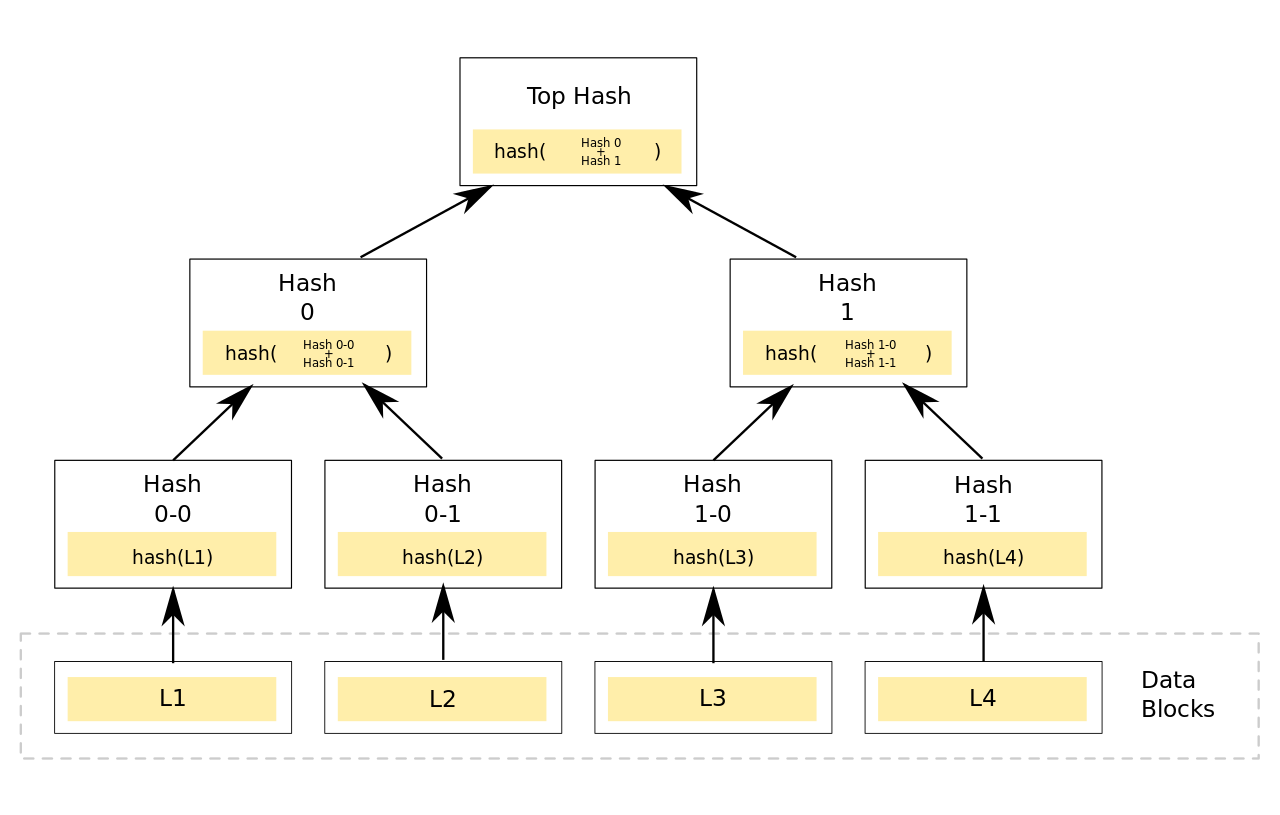
\includegraphics[width=.8\textwidth]{logo-108.png}
	\caption{Merkle树示意图}
\end{figure}

Merkle DAG的主要特点是可以在非叶子节点存储数据,并且不需要进行树的平衡操作。此外,树在面临子树重复出现时浪费了存储空间,此时使用DAG可以实现对相同子树的共享。Merkle DAG相关操作有创建、更新、插入、删除、遍历,算法上与普通有向无环图的操作一致,可以使用深度优先搜索和广度优先搜索进行遍历,故不赘述。下面以在IPFS系统中创建数字媒体作品为例展示算法流程:

step1: 对数字媒体作品切块处理,之后对数据块做hash运算,$Node_{0i}=hash(Data_{0i}),i=1,2,3,...,n,j=1$

step2:相邻两个hash块串联,然后做hash运算,$Node_{j(\frac{i+1}{2})}=hash(Node_{(j-1)i}+Node_{(j-1)(i+1)})$

step3: $j=j+1$,重复step2,直至得到根节点为止

step4:得到根节点,Merkle DAG生成完毕,算法复杂度为$O(n)$,最小生成树的长度为$log(n)+1$。

IPFS主要使用Merkle DAG进行文件存储。它将文件分成若干小块,每个块被赋予唯一的加密哈希。Markle DAG通过合并子树可以删除具有相同哈希值的节点,并跟踪每个文件的版本历史记录。查找文件时,通过文件的哈希值就可以在网络查找到储存该文件块的节点,找到想要的文件。

\subsubsection{BitSwap数据传输协议}
IPFS系统不仅包括文件存储,它在BitTorrent的基础上实现了p2p数据交换协议BitSwap。跟BitTorrent不一样的是:BitSwap获取数据块的时候不限于同一个torrent。从全局考虑,这使得BitSwap的效率更高。

为鼓励节点多分享数据,BitSwap提出信用体系:(1)节点记录自己与其他节点的传输平衡状况;(2)节点传输给负债节点数据的概率随负债的增加而减少。信用体系因不同的传输对象而异,在本模型中,为了同时保证数字媒体资源具有较高的下载速度,取BitSwap负债率的定义如下:

\[ 
r=\sqrt{\dfrac{|\dfrac{bytes\_sent}{1G}|}{|\dfrac{bytes\_recv}{1G}|+1}}
\]
\[
P(send|r) = 0.8*(1 - \dfrac{1}{1+e^{6-3r}})+0.2 
\]

其中$byte\_sent$为该节点发送的数据,$byte\_recv$为该节点接受的数据,r为负债率,$P(send|r)$为负债率为r时发送数据给该节点的概率。

\begin{figure}[!h]
	\centering
	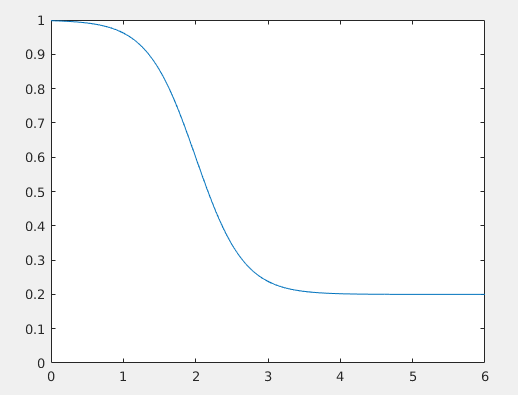
\includegraphics[width=.5\textwidth]{untitled.png}
	\caption{发送率随负债率变化曲线}
\end{figure}

如果把IPFS用户打开默认的上传功能,且仅仅上传刚接收到的数据,则$r\equiv1$,数据发送率高于90\%,如果继续转发接受的数据,则数据发送率将达到95\%以上,系统是稳定的。若节点上传接受数据的1/4则可以保持80\%的下载速度。若IPFS节点一直拒绝发送,则累计下载4G文件后下载速度减半,累计下载9G文件后没有下载加成,下载速度只有全网的20\%。

\subsubsection{IPFS可行性分析}
由于传播数字媒体时往往伴随着较高的下载量和较低的上传量,故在本模型中上传是一种被奖励的行为,奖品是更高的上传速度,而不是原BitSwap协议中要求的必需品。同时去中心化的Merkle DAG存储模式节约了大量的储存空间并且整合利用了闲置资源,这符合现代数字媒体体积大下载量高的特点,同时,Merkle DAG模式使得完整的数字媒体以碎片化的形式保存到第三方服务器上,更安全地保护了数字媒体版权,故采用IPFS系统存储数字媒体是可行的。

\section{IPTC区块生成}

在IPTC区块链中,数据会以文件的形式被永久记录,我们称这些文件为区块。一个区块是一些或所有最新知识产权交易的记录集,且未被其他先前的区块记录。新区块会被加入到记录的最后,一旦写上,就再也不能改变和删除。每个区块记录了它被创建之前发生的所有事件。一个完整的IPTC区块由下面几部分组成:区块头,区块大小,交易计数器和交易(区块主体)。

\begin{figure}[!h]
	\centering
	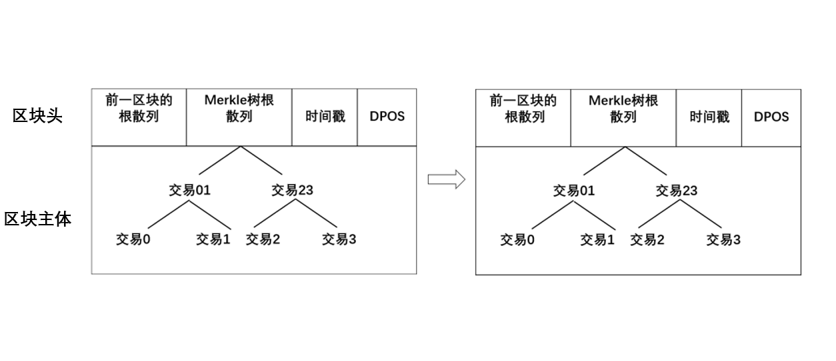
\includegraphics[width=1\textwidth]{IPTC.png}
	\caption{IPTC区块在时间上的分布}
\end{figure}

\begin{table}[h]
	\caption{IPTC区块组成结构}\label{tab001} \centering
	\begin{tabular}{ccc}
		\toprule[1.5pt]
		字节 & 字段 & 说明 \\
		\midrule[1pt]
		4 & 区块大小 & 用字节表示的该字段之后的区块大小\\
		80 & 区块头 & 组成区块头的几个字段\\
		1-9 & 交易计数器 & 该区块包含的知识产权交易数量\\
		不定 & 交易 & 记录在区块里的交易信息,使用知识产权交易信息格式,\\
		& & 分为RT、AT和PT,并且交易在数据流中的位置\\
		& & 必须与Merkle树的叶子节点顺序一致\\
		\bottomrule[1.5pt]
	\end{tabular}
\end{table}
IPTC的区块大小目前被严格限制在1MB以内,其中4字节的区块大小字段不包含在此内。

\newpage

\begin{table}[h]
	\caption{IPTC区块头结构}\label{tab001} \centering
	\begin{tabular}{ccc}
		\toprule[1.5pt]
		字节 & 字段 & 说明 \\
		\midrule[1pt]
		4 & 版本 & 区块版本号,表示本区块遵守的验证规则\\
		32 & 父区块头哈希值 & 前一区块的哈希值,使用SHA256(SHA256(父区块头))计算\\
		32 & Merkle根 & 该区块中交易的Merkle树根的哈希值,\\
		& & 同样采用SHA256(SHA256())计算\\
		4 & 时间戳 & 该区块产生的近似时间,精确到秒的UNIX时间戳\\
		4 & 难度目标 & 该区块工作量证明算法的难度目标,由DPoS机制决定\\
		\bottomrule[1.5pt]
	\end{tabular}
\end{table}
IPTC区块头中,版本信息、父区块头哈希值和Merkle根采用的是小端格式编码,即低有效位放在前面。
时间戳表示的是自1970年1月1日0时0分0秒以来的秒数,1231731025秒转为十六进制值为0x496AB951,然后采用小端格式编码表示为0x51b96a49。IPTC区块主体由众多交易组成,每一笔交易结构如下:

\begin{table}[H]
	\caption{IPTC区块交易结构}\label{tab001} \centering
	\begin{tabular}{ccc}
		\toprule[1.5pt]
		字节 & 字段 & 说明 \\
		\midrule[1pt]
		4 & 交易ID & 用于定位交易\\
		4 & 交易类型 & 用于决定采用何种交易记录方式\\
		32 & MediachainID & 作品在IPFS中的哈希\\
		32 & userID & 用户的哈希\\
		32 & pubKey & 用户的公匙(注册时出现)\\
		32 & publisherID & 发行商的哈希\\
		32 & payID & 付款方的哈希\\
		32 & recvID & 收款方的哈希\\
		4 & 授权类型 & 有A,B,C三种用于区分授权\\
		4 & Payment & 付款的数额\\ 
		32 & paySign & 付款方的签名\\
		32 & recvSign & 收款方的签名\\
		32 & paySign & 付款方的签名\\
		32 & Signature & 版权方的签名\\
		4 & 时间戳 & 该区块产生的近似时间,精确到秒的UNIX时间戳\\
		64 & Merkle索引 & 用于确定交易所处与的Merkle树位置\\
		\bottomrule[1.5pt]
	\end{tabular}
\end{table}

\end{document}